
\section{Platinen Aufbau}
Die Platine ist mit mehreren Bauteilen ausgestattet, die bis auf drei selbstdimensionierten Widerständen
bereits vollständig bestückt ist. \\
% Auf dem Schaltplan  (R Widerstand, C Kondensator, J Stecker/Relais)% 
\\
Zur Erkärung von Abbildung 4.1 hier eine kurze Information zu den wichtigsten Abkürzungen:
\begin{itemize}
    \item R: Widerstand
    \item C: Kondensator
    \item J: Stecker/Relais

    
\end{itemize}
%mache wir die Bilder 1-3 auch rein?
Die wichtigsten Bauteile sind:
%Frage: Generell wichtig oder nur für das was wir bei diesem Versuch machen? USB Buchse hier irrelevant....
\begin{itemize}
    \item J1: Anschluss an den FieldFox (Ausgangssignal)
    \item J40: Verbindung zu Oszillator (Taktquelle für die Schaltung) und Anschluss an den FiedFox (Eingangssignal)
    \item R47-49: Widerständ zur Arbeitspunkteinstellung
    \item Oszillator (XLL536C50.000000X): HF-Taktsignal
    \item Transistor (BFR181W) 
    \item Operationsverstärker (U20-LMV651MG/NOPB; U21-NCX2200GW,125)
    \item USB UART IC (FT232RL)
\end{itemize}

\begin{figure}[h]
    \centering
    \includegraphics[width=1.0\textwidth]{Pictures/Bestückungsplan.jpg}
    \caption{Bestückungsplan}
\end{figure}



\section{Bestückung PCB}
Die in Kapitel 3 bestimmten Widerstände werden nun im Rahmen der praktischen Umsetzung der Schaltung auf die 
bereits vorbereitete Platine angebracht. Auf dem Bestückungsplan entspricht hier R47 R3 mit 1000 Ohm, R48 R4 mit 
4700 Ohm und R49 R5 mit 330 Ohm. Bei dem Löten der drei Widerständen wird auf eine saubere und präzise Löttechnik
geachtet um die gewollte elektrische, mechanische und HF-technische Funktion der Schaltung zu garantieren. 
\begin{figure}[h]
    \centering
    \includegraphics[width=0.54
    \textwidth]{Pictures/Platinebestückt.jpg}
    \caption{Bestückungsplan}
\end{figure}


\section{DC-Pegel Verifizieren}
Nach dem Bestücken der Platine wird die Funktionalität der Schaltung überprüft. Hierzu wird eine Versorgungsspannung von 
4.8V angelegt um den Gleichspannungspegel an den relevanten Punkten der Schaltung zu überprüfen. Die abfallenden 
Spannungen werden mit einem Oszilloskop gemessen. Releavnt sind die Spannungsabfälle über R47, R48 und R49. Diese gemessenen
Spannungen werden mit den idealen Werten 
der Simulation verglichen. 

\section{SOLT-Kalibrierung}
Das Ziel der SOLT-Kalibrierung (Short, Open, Load, Through) ist die elemenierung
von systematischen Messfehlern. Die durch die Messausrüstung(Kabel,Adapter, etc.)
selbst entstehen und die Messung verfälschen.
Durch Messen von diesen Fehlern lässt sich die Messung korrigieren.
Dafür werden vier verschiedene Kalibrierstandards benötigt:
\begin{itemize}
    \item Short (Kurzschluss): Ein Kurzschluss-Standard wird an den Messport des VNAs angeschlossen. Da ein idealer Kurzschluss alle Leistung reflektiert und eine Phasenverschiebung von 180 Grad verursacht, misst der VNA diese Referenz. Abweichungen vom Ideal werden erfasst. 
    \item Open (Leerlauf): Ein Leerlauf-Standard wird angeschlossen. Ein idealer Leerlauf reflektiert ebenfalls die gesamte Leistung, jedoch mit einer Phasenverschiebung von 0 Grad. Auch hier werden Abweichungen aufgezeichnet.
    \item Load (Abschluss/Last): Ein Präzisions-Abschlusswiderstand (meist 50 Ohm) wird angeschlossen. Ein idealer Abschlusswiderstand absorbiert die gesamte Leistung ohne Reflexion. Dies dient dazu, die Leistungsanpassung des Systems zu kalibrieren.
    \item Through (Durchgang): Bei einer 2-Port-Messung wird ein direkter Durchgang (ein kurzes, bekanntes Kabel oder ein Adapter) zwischen den beiden Messports des VNAs angeschlossen. Dies ermöglicht die Kalibrierung der Übertragungseigenschaften zwischen den Ports und die Korrektur von Phasen- und Amplitudenfehlern des Übertragungspfades.
\end{itemize}
\clearpage

%(erklärung warums tut)
\begin{figure}[h]
    \centering
    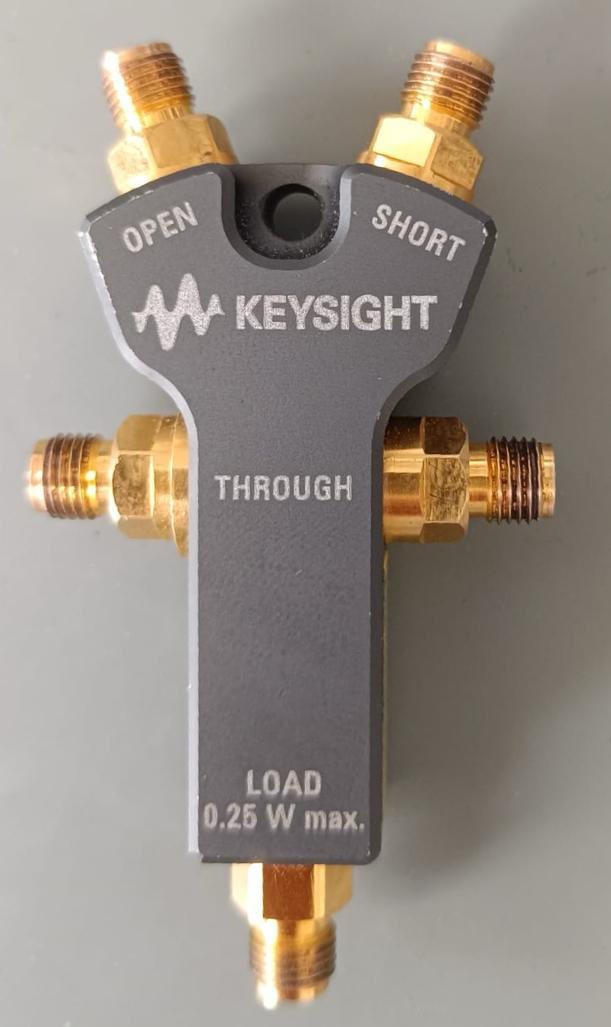
\includegraphics[width=0.35\textwidth]{Pictures/Keysightkallibrierung.jpg}
    \caption{Bestückungsplan}
\end{figure}
Die Kalibierung wird an dem Keysight FieldFox durchgeführt. Sie erfolgt über sieben Schritte die von dem Gerät 
angeleitet werden. Danach ist das Gerät bereit für die Messung.

\section{Vergleich zur Simulation}
Die Simulation wurde, wie zuvor beschrieben, mit der Sofrware Adcanced Design System (ADS) durchgeführt. In der Simulation fällt über R47 eine Spannung
von 0,811 V, bei R48 eine Spannung von 3,989 V und bei R49 eine Spannung von 1,27 V ab. Wir überprüfen nun ob sich unsere Messung mit den simulierten Werten
deckt.
\\

\begin{table}[h]
    \centering
    \begin{tabular}{|l|l|l|}
        \hline
        \textbf{Widerstand} & \textbf{Simulation [V]} & \textbf{Messung [V]} \\
        \hline
        R47 & 0{,}811 & 0{,}809 \\
        \hline
        R48 & 3{,}989 & 3{,}991 \\
        \hline
        R49 & 1{,}27  & 1{,}26 \\
        \hline
    \end{tabular}
    \caption{Vergleich von simulierten und gemessenen Spannungswerten}
\end{table}

\clearpage
